% \chapter{Locomotion and Manipulation}\label{chap:locomotion}
\chapter{运动和操作}\label{chap:locomotion}

% Autonomous robots are systems that sense, actuate, compute, and communicate. Actuation, the focus of this chapter, is the ability of the robot to move and to manipulate the world. Specifically, we differentiate between locomotion\index{Locomotion} as the ability of the robot to move and manipulation\index{Manipulation} as the ability to move objects in the environment of the robot. Both activities are closely related: during locomotion the robot uses its motors to exert forces on its environment (ground, water or air) to move itself; during manipulation it uses motors to exert forces on objects to move them relative to the environment. This might not even require different motors. Insects are good examples for this: both can use their 6 legs not only for locomotion, but also for picking up and manipulating objects. The goals of this chapter are
% \begin{itemize}
% \item introduce the concepts of locomotion, manipulation and their duality
% \item explain static vs.\ dynamic stability
% \item introduce ``degrees-of-freedom''
% \item and introduce forward kinematics of static arms.
% \end{itemize}

自主机器人是具有感知、驱动、计算和通信能力的系统。本章的重点是机器人移动和操作的能力。具体来说,运动\index{Locomotion}是机器人在其环境中移动的能力, 而操作\index{Manipulation}是机器人在其环境中移动物体的能力。这两个活动是密切相关的:在运动期间,机器人利用其电机对环境(地面、水或空气)施加力量从而自身能够移动;在操作过程中,它使用电机对物体施加力,使该物体相对于环境移动。这甚至不需要不同的电机。昆虫是很好的例子:它们的六条腿不仅可以使它们运动,还可以用于拾取和操作物体。 本章的目标是:

\begin{itemize}
\item 介绍运动、操作及其二元性的概念
\item 解释静态与动态稳定性
\item 介绍“自由度”
\item 介绍静态机械臂的正向运动。
\end{itemize}


% \section{Locomotion and Manipulation Examples}
\section{运动和操作实例}

% Locomotion includes very different concepts of motion including rolling, walking, running, jumping, sliding (undulatory locomotion), crawling, climbing, swimming, and flying. They are drastically different in terms of energy consumption, kinematics, stability, and capabilities required by the robot that implements them. Yet, the above definitions are loose and ambiguous: for example, ``swimming'' can be done using many different forms of propulsion systems. Similarly, a sliding motion on the ground might result into swimming with only few modifications.

运动包括截然不同的运动概念,包括滚动、步行、跑步、跳跃、滑动(波状运动)、爬行、攀爬、游泳和飞行。对于实现这些运动的机器人来说,不同的运动在能量消耗、运动学、稳定性和能力等方面是截然不同的。然而,上述定义是宽松和不明确的:例如,“游泳”可以使用许多不同形式的推进系统来完成。 类似地,在地面上的滑动可能只需很少的改动就可以变成游泳。

% The way in which the individual parts of a robot can move with respect to each other and the environment is called the \emph{kinematics}\index{Kinematics} of the robot. Kinematics are only concerned with the position and speed (first derivative of position) of those parts, but not its \emph{dynamics}, which include acceleration (second derivative of position) and jerk (third derivative of position).

机器人的各个部件相对于彼此和环境移动的方式称为机器人的\emph{运动学}\index{Kinematics}。运动学仅涉及这些部件的位置和速度(位置的一阶导数),而不是其\emph{动力学},包括加速度(位置的二阶导数)和混合(位置的三阶导数)。

% Commercially, the most dominant form of locomotion is rolling. This is due to the fact that rolling provides by far the most efficient energy-speed ratio (Figure \ref{fig:todd}), making the invention of the wheel one of the greatest technological breakthroughs in history. Consequently, humans have modified their environment to have smooth surfaces of large extent such as the road network, but also warehouse and residential floors. In contrast, evolution has not evolved a single animal with wheel-like actuators.

在商业中,最主要的运动形式是滚动。 这是由于滚动提供了迄今为止最有效的能量速度比(图~\ref{fig:todd}),使得轮子的发明成为历史上最大的技术突破之一。因此,人类已经改变他们的环境,以便在很大程度上形成光滑的表面,如道路网、还有仓库和住宅楼的地面。相比之下,进化并没有使任何一种动物发展出轮状的驱动器。

\begin{figure}
	\centering
		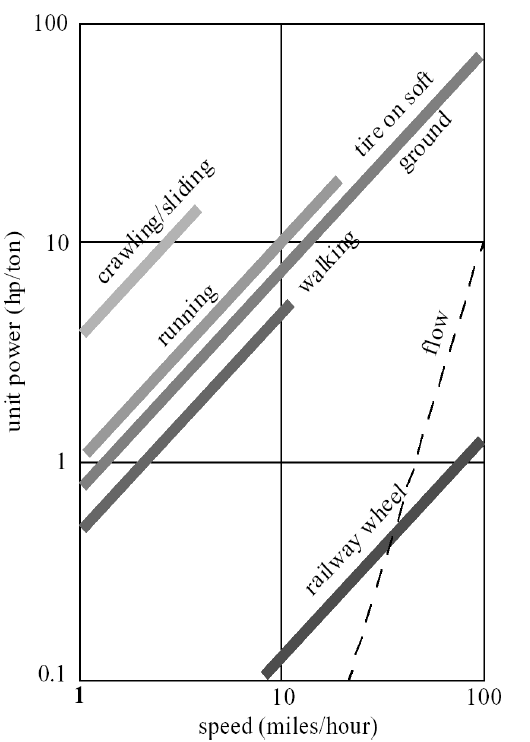
\includegraphics[width=0.8\textwidth]{figs/todd85.png}
	% \caption{Power consumption vs.\ speed for various means of locomotion. From \protect\citeasnoun{todd1985walking}.}
	\caption{不同运动的功耗与速度。 摘自\protect\citeasnoun{todd1985walking}.}
	\label{fig:todd}
\end{figure}


\begin{framed}
% Can you find examples of robots from the above categories? Identify the different types of actuators that are used in them.
你可以从上述类别中找到对应机器人的例子吗?指出它们使用的不同类型的驱动器。
\end{framed}

% Due to the dominance of rolling robots, the electric motor is among the most popular actuators. Except for the stepper motor, which uses large electromagnets to rotate an internal spindle by a few degrees every time, the physics of the electrical motor requires it to revolve at very high speeds (multiple thousand rotations per minute). Therefore, motors are almost always used in conjunction with gears to reduce the speed and increase the torque, that is the force that the motor can exert to rotate an axis. In order to be able to measure the number of revolutions and the axis' position, motors are also often combined with rotary encoders. Motors that combine an electric motor with a gear-box, encoder, and controller to move toward desired position are known as servo motors, and are popular among hobbyists. Another popular class of actuator, in particular for legged robots, are linear actuators, that might exist in electric, pneumatic or hydraulic form. Finally, there exist a wide array of specialty actuators such as Shape-Memory Alloys, Electroactive Polymers or Piezo-elements, which often allow for extreme miniaturization, but do not provide attractive energy-to-force ratios and are difficult to control.

由于轮式机器人的优势,电机是最受欢迎的驱动器之一。除了使用大型电磁铁将内部主轴每次旋转几度的步进电机外,电机的物理学需要电机以非常高的速度旋转(每分钟几千转)。因此,电机几乎总是与齿轮一起使用,以降低转速并增加扭矩,也就是电机可以施加的力使得轴旋转。为了能够测量转数和轴位置,电机也经常与旋转编码器组合。将电动机与齿轮箱、编码器和控制器组合以移动到期望位置的电机被称为伺服电机,并且在爱好者中很受欢迎。另一类受欢迎的驱动器,尤其是对于足式机器人,是可能以电动、气动或液压形式存在的驱动器。最后,存在各种各样的专业驱动器,例如形状记忆合金、电活性聚合物或压电元件,其通常允许极小型化,但能量-力度比较低,并且难以控制。

% Most actuators (and mechanisms) capable of locomotion can also be used for manipulation with only minor modifications. Most industrial manipulators consist of a chain of rotary actuators that are connected by links. Most industrial robots have six or more independently rotating axes. We will see why further down below. Modern industrial manipulators have the ability to not only control the position of each of its joints, but precisely control the torque and force at each individual joint, making the arm arbitrary compliant, which is the inverse of stiffness in a mechanical sense. For dexterous manipulation a robot does not only need an arm, but also a gripper or hand. Grasping is a hard problem on its own and deserves its own chapter. 

仅进行微小修改,大多数用来运动的驱动器(和机械)也可以用于操作。大多数工业操作臂由通过连杆连接的旋转驱动器链组成。大多数工业机器人具有六个或更多的独立旋转轴。我们会看到为什么数量进一步减少。现代工业操作臂不仅能够控制每个关节的位置,而且可以精确地控制每个单个关节处的扭矩和力,从而使操作臂任意顺从,这与机械意义上的刚度相对应。对于灵巧操作,机器人不仅需要操作臂,而且还需要夹子或手。 抓取本身就是一个难题,值得独自成章。

%% Start - Was commented
%This lecture focuses on the kinematics of simple mechanisms. Understanding the duality between locomotion and manipulation is important, however, to better introduce (and understand) concepts such as reference frames and forward kinematics.
%% End - Was commented

% \section{Static and Dynamic Stability}\label{sec:stability}
\section{静态和动态稳定性}\label{sec:stability}

% A fundamental difference between locomotion mechanisms is whether they are statically or dynamically stable\index{Static stability}\index{Dynamic Stability}. A statically stable mechanism will not fall even when all of its joints freeze (Figure \ref{fig:stability}, left). A dynamically stable robot instead requires constant motion to prevent it from falling. Technically, stability requires the robot to keep it's center of mass to fall within the polygon spanned by its ground-contact points. For example a quadruped robot's feet span a rectangle. Once such a robot lifts one of its feet, this rectangle becomes a triangle. If the projection of the center of mass of the robot along the direction of gravity is outside of this triangle, the robot will fall. A dynamically stable robot can overcome this problem by changing its configuration so rapidly that a fall is prevented. An example of a purely dynamically stable robot is an inverted pendulum on a cart (Figure \ref{fig:stability}, middle). Such a robot has no statically stable configurations and needs to keep moving all the time to keep the pendulum upright. While dynamic stability is desirable for high-speed, agile motions, robots should be designed so that they can easily switch into a statically stable configuration (Figure \ref{fig:stability}, right). 

运动机制之间的根本区别在于它们是静态稳定还是动态稳定\index{Static stability}\index{Dynamic Stability}。即使其所有关节都静止,静态稳定的构造也不会崩塌(图~\ref{fig:stability},左)。动态稳定的机器人需要恒定的运动来防止其跌倒。从技术上讲,稳定性要求机器人将其质心保持在由其触地点覆盖的多边形内。例如四足机器人的脚组成矩形。一旦这样的机器人抬起一只脚,这个矩形就变成三角形。如果机器人沿重力方向的质心投影在三角形之外,机器人将会跌倒。动态稳定的机器人可以通过快速改变其构造来克服这个问题,防止跌倒。小推车上倒立的摆锤就是一个纯动态稳定的机器人的例子(图~\ref{fig:stability},中间)。这样的机器人没有静态稳定的构造,需要始终保持移动以保持摆锤的直立。虽然动态稳定性对于高速、敏捷的运动是需要的,但是机器人应该被设计成使得它们可以容易地转换成静态稳定的构造(图~\ref{fig:stability},右)。

\begin{figure}
	\centering
		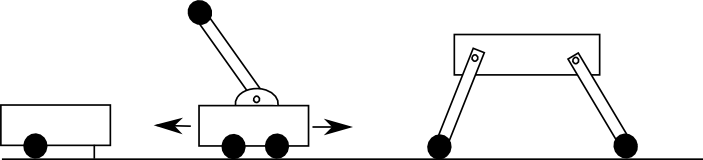
\includegraphics[width=\textwidth]{figs/stability.png}
	% \caption{From left to right: statically stable robot. Dynamically stable inverted pendulum robot. Static and dynamically stable robot (depending on configuration).}
	\caption{从左到右:静态稳定的机器人。动态稳定的倒立的摆锤。 静态和动态稳定的机器人(取决于构造)。}
	\label{fig:stability}
\end{figure}

% An example of a robot that has both statically and dynamically stable configurations is a quadruped (``four legs'') runner. Unlike walking, a running robot will always have two legs in the air and alternate between them faster than the robot could fall in either direction. Although statically stable walking is possible with only 4 legs, most animals (and robots) require 6 legs for statically stable walking and use dynamically stable gaits (such as galloping) when they have four legs. Six legs allow the animal to move three legs at a time while the three other legs maintain a stable pose.

四足(“四条腿”)跑步者是一个同时具有静态稳定和动态稳定构造的机器人的例子。与步行不同的是,一个运动中的机器人总是有两条腿在空中,两腿与两腿交替的速度比机器人快会使机器人向任一方向跌倒。虽然只需四条腿就可以稳定行走,但大多数动物(和机器人)需要六条腿用于静态稳定的行走,并且当它们只有四条腿时使用动态稳定的步态(例如奔跑)。六条腿允许动物一次移动三条腿,而另外三条腿保持稳定的姿势。

% \section{Degrees-of-Freedom}\label{sec:dof}
\section{自由度}\label{sec:dof}

% The concept of \emph{degrees-of-freedom}\index{Degree of freedom}, often abbreviated as DOF, is important for defining the possible positions and orientations a robot can reach. An object in the physical world can have up to six degrees of freedom, namely forward/backward, sideways, and up/down as well as rotations around those axes. These rotations are known as pitch, yaw and roll and are illustrated in Figure \ref{fig:pitchyawandroll}. 

通常缩写为DOF的\emph{自由度(Degree of Freedom)}\index{degree of freedom}的概念对于定义机器人可能达到的位置和方向很重要。 物理世界中的一个物体可以具有六个自由度,即前进/后退、侧向、上/下以及这些围绕轴的旋转。这些旋转称为俯仰(pitch)、偏航(yaw)和滚动(roll),并在图~\ref{fig:pitchyawandroll}中说明。

\begin{figure}
	\centering
		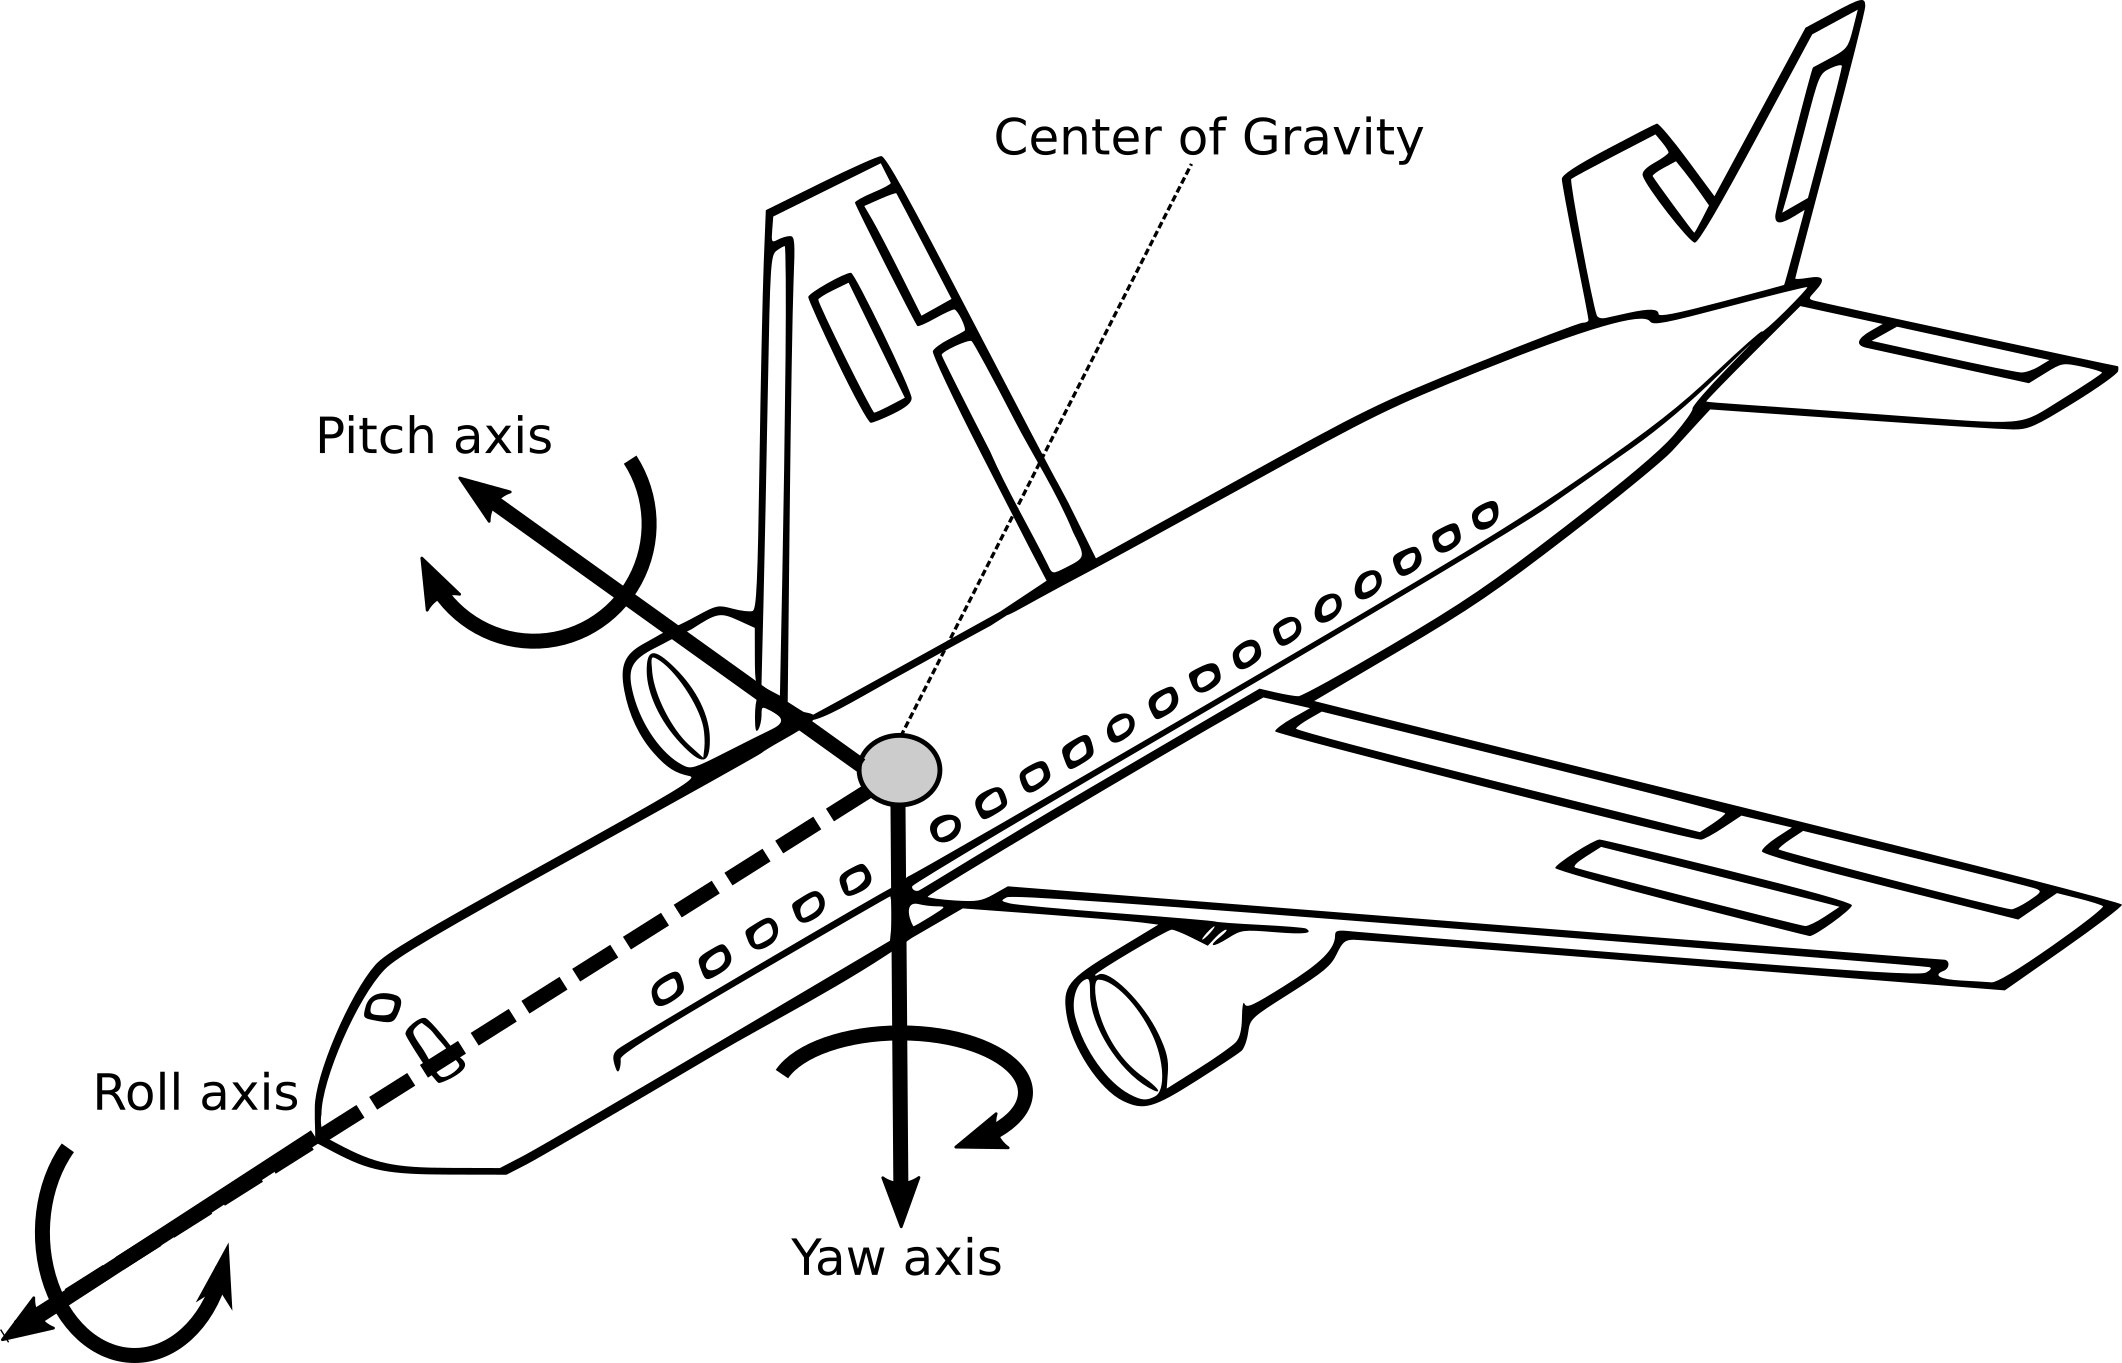
\includegraphics[width=\textwidth]{figs/pitchyawroll.png}
	% \caption{Pitch, yaw and roll around the principal axis of an airplane.}
	\caption{绕飞机主轴的俯仰(pitch)、偏航(yaw)和滚动(roll)。}
	\label{fig:pitchyawandroll}
\end{figure}

% How many of those directions a robot can move in depends on the configuration of its actuators and the constraints the robot has with the environment. These relationships are not always intuitive and require more rigorous mathematical treatment (Chapter \ref{chap:kinematics}). The goal of this section is to introduce the degrees of freedom of standard mechanisms that are recurrent in robot design such as wheels or simple arms. For wheeled platforms, the degrees-of-freedom are defined by the types of wheels used and their orientation. Common wheel types are listed in Table \ref{tab:wheels}.

在不同方向上机器人可以移动多少取决于其驱动器的构造和机器人与环境间的约束。这些关系并不总是直观的,它们需要更严格的数学处理(第\ref{chap:kinematics}章)。 本部分的目标是介绍机器人设计中反复出现轮子或简单机械臂的标准构造的自由度。对于轮式平台,自由度由所使用的轮子类型及其方向定义。 常见的轮子类型列在表\ref{tab:wheels}中。

% \begin{table}
% \begin{tabular}{p{2.8cm}p{3cm}p{4cm}}
% \hline
% Wheel type & Example & Degrees-of-Freedom\\
% \hline
% Standard 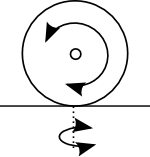
\includegraphics[width=2.5cm]{figs/wheeltype_standard.png} &	Front-wheel of a wheelbarrow	& Two
% \begin{compactitem}
% \item Rotation around the wheel axle
% \item Rotation around its contact point with the ground
% \end{compactitem}\\
% \hline
% Caster wheel	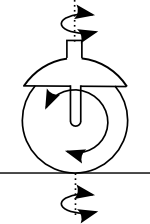
\includegraphics[width=2.5cm]{figs/wheeltype_caster.png}& Office chair & Three
% \begin{compactitem}
% \item Rotation around the wheel axle
% \item Rotation around its contact point with the ground
% \item Rotation around the caster axis
% \end{compactitem}\\
% \hline
% Swedish wheel 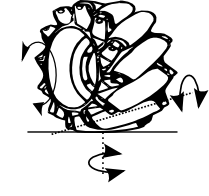
\includegraphics[width=2.5cm]{figs/wheeltype_swedish.png}& Standard wheel with non-actuated rollers around its circumference& Three
% \begin{compactitem}
% \item Rotation around the wheel axle
% \item Rotation around its contact point with the ground
% \item Rotation around the roller axles
% \end{compactitem}\\
% \hline
% Spherical wheel 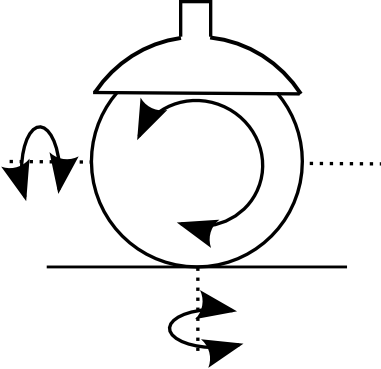
\includegraphics[width=2.5cm]{figs/wheeltype_spherical.png}& Ball Bearing & Three
% \begin{compactitem}
% \item Rotation in any direction
% \item Rotation around its contact point
% \end{compactitem}\\
% \hline
% \end{tabular}
% \caption{Different types of wheels and their degrees of freedom. Adopted from \protect\citeasnoun{siegwart2011introduction},\label{tab:wheels}}
% \end{table}

\begin{table}
\begin{tabular}{p{2.8cm}p{3cm}p{4cm}}
\hline
轮子类型 & 例子 & 自由度\\
\hline
标准 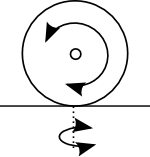
\includegraphics[width=2.5cm]{figs/wheeltype_standard.png} & 独轮车的前轮	 & Two
\begin{compactitem}
\item 围绕轮轴旋转
\item 围绕其与地面接触点旋转
\end{compactitem}\\
\hline
脚轮	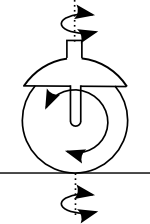
\includegraphics[width=2.5cm]{figs/wheeltype_caster.png}& 办公椅 & Three
\begin{compactitem}
\item 围绕轮轴旋转
\item 围绕其与地面接触点旋转
\item 围绕脚轮轴旋转
\end{compactitem}\\
\hline
瑞典轮 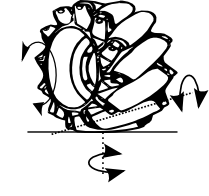
\includegraphics[width=2.5cm]{figs/wheeltype_swedish.png}& 周围有非驱动滚轴的标准轮 & Three
\begin{compactitem}
\item 围绕轮轴旋转
\item 围绕其与地面接触点旋转
\item 围绕滚轴旋转
\end{compactitem}\\
\hline
球形轮 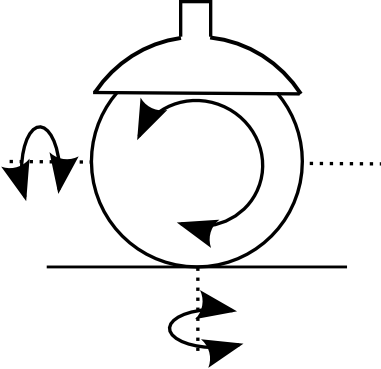
\includegraphics[width=2.5cm]{figs/wheeltype_spherical.png}& 球轴承 & Three
\begin{compactitem}
\item 围绕任意方向旋转
\item 围绕其与地面接触点旋转
\end{compactitem}\\
\hline
\end{tabular}
\caption{不同类型的车轮及其自由度。摘自\protect\citeasnoun{siegwart2011introduction}
\label{tab:wheels}}
\end{table}


% Only robots that use exclusively wheels with three degrees-of-freedom (3-DOF wheels) will be able to freely move on a plane. This is because the pose of a robot on a plane is fully given by its position (two values) and its orientation (one value). Robots that don't have wheels with three degrees of freedom will have \emph{kinematic constraints}\index{Kinematic constraints} that prevent them from reaching every possible point at every possible orientation. For example, a bicycle wheel can only roll into one direction and turn on the spot. Moving the bicycle wheel orthogonal to its direction of rolling is not possible, unless it is forcefully dragged (``skidding''), which requires more involved treatment not covered in this book. On the other hand, not having three degrees of freedom does not mean that not all poses in the plane can be reached. 

只有使用三自由度的轮子(3-DOF轮)的机器人能够在平面上自由移动。这是因为机器人在平面上的姿态由其位置(两个值)及其方向(一个值)完全确定。没有具有三自由度的轮子的机器人有阻止它们在任一可能的方向到达任一可能点的\emph{运动约束}\index{Kinematic constraints}。例如,自行车车轮只能向一个方向滚动并沿着触地点转动。沿着自行车车轮与其滚动方向正交的方方向移动是不可能的,除非车轮被外力拽动(“打滑”),这需要本书中不涉及的更多相关知识。另一方面,没有三自由度并不意味着平面上的所有姿态(位置+方向)都达不到。

% A good analogue are figures on a chess-board. For example, a knight can reach every cell on a chess-board but might require multiple moves to do so. This is similar to a car, which can parallel park using back-and-forth motions. Instead, a bishop can only reach either black or white fields on the board. 

我们用国际象棋棋盘上的角色打比方。例如,“骑士”可以到达棋盘上的每个格,但是可能需要执行多个动作。这类似于一辆通过前后运动来并排停车的汽车。相反,“主教”只能到达板上的黑色或白色的区域。

% Similar reasoning applies to aerial and underwater robots. Here, the position of the robot is affected by the position and orientation of thrusters, either in the form of jets or propellers, mounted on the robot. Things become complicated quickly, however, as the dynamics of the system are subject to fluid- and aerodynamic effects, which also change as a function of size of the robot. This book will not go into the details of flying and swimming robots, but the general principles of localization and planning will be applicable to them as well.

类似的推理适用于空中和水下机器人。这里,机器人的位置受安装在机器人上的推进器的位置和方位的影响,比如喷射器或螺旋桨。然而,事情很快变得复杂,因为系统的动力学受到流体和空气动力学效应的影响,这也随着机器人的尺寸而变化。虽然本书不会涉及飞行和游动机器人的细节,但定位和规划的一般原则仍适用于它们。

\begin{framed}
% Think about possible wheel, propeller and thruster configurations. Don't limit yourself to robots, but consider also street and aerial vehicles and be creative --- if you can think about a setup that makes sense, i.e., allows for reasonable mobility --- somebody will already have built it and analyzed it. What are the advantages and disadvantages of each?
想想可能的轮子、螺旋桨和推进器构造。不要局限于机器人,也要考虑街上和空中交通工具,发散思维(如果你可以想到一个有意义的构造,即允许合理的机动性,那么有人已经建造并分析过了)。 每个的优点和缺点是什么?
\end{framed}

% For manipulating arms, degrees of freedom usually refer to the positions and orientations, i.e., rotations around the primary axes, the end-effector can reach. As a rule of thumb, each joint usually adds a degree of freedom unless they are redundant, that is, moving in the same direction. Figure \ref{fig:basickinematics} shows a series of manipulators operating in a plane. By this, the degrees of freedom of the end-effector are limited to moving up and down, sideways, and rotating around its pivot point. As a plane only has those three degrees of freedom, adding additional joints cannot increase the degrees of freedom unless they allow the robot to also move in and out of the plane. 

% An exact definition of the number of degrees of freedom is tricky and requires deriving analytical expressions for the end-effector position and orientation, which will be subject to Chapter \ref{chap:kinematics}.

对于操作臂,自由度通常指的是位置和方向,即围绕主轴的转动,末端执行器可以达到。根据经验,除非是多余的,即沿相同的方向移动,每个关节通常会增加一个自由度。 图\ref{fig:basickinematics}显示了一系列在平面上操作的操作臂。由此,末端执行器的自由度被限制为上下移动、侧向移动并绕其转轴旋转。由于一个平面只有三个自由度,所以添加额外的关节不能增加自由度,除非我们允许机器人能进出平面。

准确算出自由度多少是棘手的,需要得出末端执行器位置和方向的解析表达式,这会在第\ref{chap:kinematics}章介绍。

\begin{figure}
	\centering
		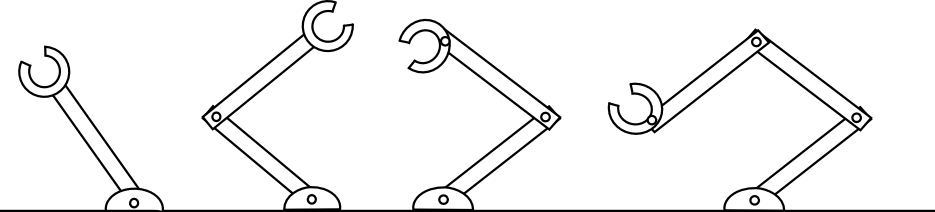
\includegraphics[width=\textwidth]{figs/basickinematics.png}
	% \caption{From left to right: Manipulators with one, two, three and three DOF. The degrees of freedom of moving in a plane are the position of the end-effector with respect to its height and displacement with respect to the base, as well as its orientation.}
	\caption{从左到右:有一个、两个、三个和三自由度的操作臂。在平面中移动的自由度包括末端执行器相对于其高度的位置、其相对于基座的位移及其方向。}
	\label{fig:basickinematics}
\end{figure}

% Choosing the ``right'' kinematics is a trade-off between mechanical complexity, maneuverability, achievable precision, cost, and ease of control. The very popular differential-wheel drive consisting of two independently controlled wheels that share a common axis such as on the iRobot Roomba is cheap, highly maneuverable and easy to control, but makes it hard to drive in a straight line. This requires both motors to turn at the exact same speed and both wheels to have the exact same diameter, which is hard to achieve in practice. This problem is solved well by car-like steering mechanisms, but they have poor maneuverability and are difficult to control (think parallel-parking).

选择“正确”运动学需要在机械复杂性、机动性、可实现的精度、成本和易于控制之间作权衡。非常受欢迎的差动轮驱动器由两个独立控制的车轮组成,这两个车轮共享一个共同的轴线,如iRobot Roomba,便宜、高度机动性和易于控制,但这样的设计使其难以直线行进。这需要两个电机以完全相同的速度转动,并且两个车轮具有完全相同的直径,这在实践中很难实现。这类问题可以利用汽车式转向原理得到很好的解决,但是这种方法机动性差、难以控制(考虑平行停车)。

% \section*{Take-home lessons}
\section*{课后补充}

% \begin{itemize}
% \item In order to do planning for a robot, you need to understand how its control parameters map to actions in the physical world.
% \item The kinematics of a robot are fully defined by the position and orientation of its wheels, joints and links no matter whether it swims, flys, crawls or drives.
% \item Many robotic systems cannot be fully understand by considering kinematics alone, but require you to model their dynamics as well. This book will be limited to modeling kinematics, which is sufficient for low-speed, mobile robots and arms.
% \end{itemize} 

\begin{itemize}
\item 为了对机器人进行规划,你需要了解其控制参数如何映射到物理世界中的动作。
\item 机器人的运动学完全由其轮子、关节和链接的位置和方向决定,无论它是游泳、飞行、爬行还是驾驶。
\item 对许多机器人系统来说,仅考虑运动学,你并不能完全理解,也需要你对其动力学建模。本书仅限于运动学建模,这对于低速、移动机器人和操作臂是足够的。
\end{itemize} 

% \section*{Exercises}\small
% \begin{enumerate}
% \item What are the degrees of freedom of a lawnmower with four standard wheels? Why are you still able to mow your entire lawn?
% \item Is a car statically or dynamically stable? What about a Segway?
% \item What are the degrees of freedom of an office chair with all caster-wheels?
% \item What are the maximum degrees of freedom for objects driving on the plane?
% \item What are the maximum degrees of freedom for objects that can freely move in the world?
% \item Calculate the degrees of freedom of a differential wheels robot with a front caster wheel. What happens when you add a second caster wheel?
% \item Calculate the degrees of freedom of a standard car. How can you still reach every point on the plane?
% \item A steering wheel allows you to change the yaw of your car. Can you also change its pitch and its roll?
% \end{enumerate}\normalsize

\section*{习题}\small
\begin{enumerate}
\item 具有四个标准轮的割草机的自由度是多少? 为什么你还能修剪整个草坪?
\item 汽车是静态稳定还是动态稳定? Segway呢?
\item 有全部脚轮的办公椅的自由度是多少?
\item 平面上驾驶的物体的最大自由度是多少?
\item 世界上可以自由移动的物体的最大自由度是多少?
\item 计算带有前脚轮的差动轮机器人的自由度。 如果你加第二个脚轮会发生什么?
\item 计算标准汽车的自由度。 你怎样达到平面上的每一点?
\item 方向盘允许你改变汽车的偏航(yaw)。 你是否也可以改变它的俯仰(pitch)和滚动(roll)?
\end{enumerate}\normalsize